\begin{exercise}
      {ID-bd2471708d3f765a90ce138637c8bf3e4703e586}
      {High Noon}
  \ifproblem\problem\par
    In den beiden Orten $A$ und $B$ brechen zur selben Zeit zwei Fahrradfahrer auf.
    Der Fahrradfahrer, der in $A$ startet, fährt nach $B$, und der Fahrradfahrer, der
    in $B$ startet, fährt nach $A$. Sie benutzen denselben Weg und treffen sich genau um
    12:00 Uhr mittags.
    \begin{center}
      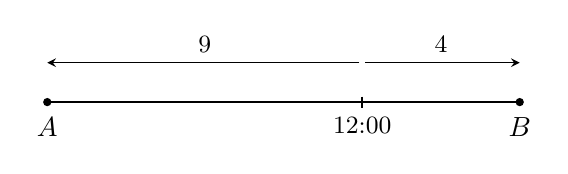
\begin{tikzpicture}
        % Weg
        \draw[line width=0.6pt] (0, 0) -- (6, 0);
        % Punkte
        \fill[fill=black] (0, 0) circle[radius=1.5pt] node[below=2pt]{$A$};
        \fill[fill=black] (6, 0) circle[radius=1.5pt] node[below=2pt]{$B$};
        % Markierung: 12:00
        \draw[line width=0.6pt] (4, 2pt) -- (4, -2pt) node[below]{\small12:00};
        % Pfeil: 9h
        \draw[line width=0.4pt, ->, >=stealth, shorten <=1pt]
             (4, 5mm) -- node[above]{\small\SI{9}{\hour}}
             (0, 5mm);
        % Pfeil: 4h
        \draw[line width=0.4pt, ->, >=stealth, shorten <=1pt]
             (4, 5mm) -- node[above]{\small\SI{4}{\hour}}
             (6, 5mm);
      \end{tikzpicture}
    \end{center}
    Nachdem sie sich begegnet sind, braucht der eine Fahrradfahrer noch 4
    Stunden bis er in $B$, und der andere Fahrradfahrer noch 9 Stunden bis
    er in $A$ angekommen ist. Wann sind die beiden Fahrradfahrer aufgebrochen?
  \fi
  \ifoutline\outline\par
    Ausgangspunkt für die Lösung dieser Aufgabe ist der Zusammenhang
    zwischen Weg $s$, Zeit $t$ und Geschwindigkeit $v$:
    \begin{equation*}
      s=v\cdot t
    \end{equation*}
    Aus der Aufgabenstellung geht hervor, dass der erste Fahrradfahrer,
    der von $A$ nach $B$ fahrt, nachmittags in 4 Stunden mit seiner
    Geschwindigkeit dieselbe Strecke zurückgelegt hat, wie der zweite
    Fahrradfahrer am Vormittag.
    Und der zweite Fahrradfahrer, der von $B$ nach $A$ fährt, legt
    nachmittags in 9 Stunden mit seiner Geschwindigkeit dieselbe Strecke
    zurück, wie der erste Fahrradfahrer am Vormittag.\par
    Wenn man mit $x$ die Zeitspanne in Stunden bezeichnet, in der die
    Fahrradfahrer vormittags unterwegs waren und mit $v_{AB}$ bzw.
    $v_{BA}$ deren jeweilige Geschwindigkeit, dann gilt folgendes
    Gleichungssystem:
    \begin{equation*}
      \left|
      \begin{split}
        x\cdot v_{AB}&=9\cdot v_{BA}\\
        x\cdot v_{BA}&=4\cdot v_{AB}
      \end{split}
      \right.
    \end{equation*}
  \fi
  \ifoutcome\outcome\par
    Wenn man mit $x$ die Zeitspanne in Stunden bezeichnet, in der die
    Fahrradfahrer vormittags unterwegs waren und mit $v_{AB}$ bzw.
    $v_{BA}$ deren jeweilige Geschwindigkeit, dann gilt folgendes
    Gleichungssystem:
    \begin{equation*}
      \left|
      \begin{split}
        x\cdot v_{AB}&=9\cdot v_{BA}\\
        x\cdot v_{BA}&=4\cdot v_{AB}
      \end{split}
      \right.
    \end{equation*}\par
    Löst man die erste Gleichung nach $v_{BA}$ auf, erhält man:
    \begin{equation*}
      v_{BA}=\frac{x}{9}\cdot v_{AB}
    \end{equation*}\par
    Damit lässt sich nun die Variable $v_{BA}$ in der zweiten
    Gleichung ersetzen:
    \begin{equation*}
      x\cdot\frac{x}{9}\cdot v_{AB}=4\cdot v_{AB}
      \quad\Rightarrow\quad
      x^2=36
      \quad\Rightarrow\quad
      x=6
    \end{equation*}\par
    Die beiden Fahrradfahrer sind also um 6:00 Uhr morgens losgefahren.
  \fi
\end{exercise}
